%\documentclass[conference, oribibl]{IEEEtran}
\documentclass[runningheads,a4paper,oribibl]{llncs}
%\usepackage{llncsdoc}

% *** MISC UTILITY PACKAGES ***
%

\usepackage{amssymb}
\usepackage{verbatim}
\setcounter{tocdepth}{3}
\usepackage{adjustbox,lipsum}

\usepackage{graphicx}
\graphicspath{ {Figs/} }

\usepackage{amsmath}
\usepackage{multirow}
%\usepackage{slashbox}
\usepackage{amsfonts}

\usepackage{algpseudocode}
\usepackage{algorithm}
\usepackage{epstopdf}
\usepackage{array}
\usepackage{enumerate}

\usepackage{epstopdf}

\usepackage{url}
\usepackage{subcaption}
\captionsetup{compatibility=false}
\usepackage{hyperref}
\usepackage{wrapfig}
%\urldef{\mailsa}\path|{khanhtv, mizuhito}@jaist.ac.jp|    

%ieee requirements
%\usepackage[utf8]{inputenc}
%\usepackage[T1]{fontenc}
%\usepackage{microtype} 
%\usepackage{balance}

%user definitions
\newcommand{\Nat}{{\mathbb N}}
\newcommand{\Real}{{\mathbb R}}
\newcommand{\Rat}{{\mathbb Q}}
\newcommand{\suppress}[1]{} % Comment out text.
\newcommand{\mizuhito}[1]{\{{\bf Mizuhito:~\sf #1}\}} % Highlight text.
\newcommand{\khanh}[1]{\{{\bf Khanh:~\sf #1}\}} % Highlight text.

\newcommand{\smallHead}[1]{%
    \par\vspace{.35cm}\noindent\textbf{#1}%
    \par\noindent\ignorespaces%
}

\newcommand\TTTT{%
 \textsf{T\kern-0.2em\raisebox{-0.3em}T\kern-0.2emT\kern-0.2em\raisebox{-0.3em}2}%
}

% correct bad hyphenation here
\hyphenation{op-tical net-works semi-conduc-tor}


\begin{document}
%
% paper title
% can use linebreaks \\ within to get better formatting as desired
% Do not put math or special symbols in the title.

\title{raSAT : SMT Solver for Polynomial Constraints} 
\author{Vu Xuan Tung\inst{1}, To Van Khanh\inst{2}, and Mizuhito Ogawa\inst{1}} 
\institute{
Japan Advanced Institute of Science and Technology\\
\email{\{tungvx,mizuhito\}@jaist.ac.jp}
\and 
University of Engineering and Technology, Vietnam National 
University, Hanoi \\
\email{khanhtv@vnu.edu.vn}
}

%\tableofcontents

% make the title area
\maketitle

% As a general rule, do not put math, special symbols or citations
% in the abstract
\begin{abstract}
  This paper presents an SMT solver {\bf raSAT} for polynomial constraints, 
  which aims to handle them over both reals and integers with
  simple unified methodologies: (1) {\bf raSAT} {\em loop} for inequations,
  which extends the \emph{interval constraint propagation}
  with testing to accelerate SAT detection, and 
  (2) a non-constructive reasoning for equations over reals,
  based on the Intermediate Value Theorem. 
\end{abstract}


\section{Introduction}
{\em Polynomial constraint solving} is to find an instance that satisfies given
polynomial inequations/equations. Various techniques are implemented in SMT solvers,
e.g., for reals (\emph{QF\_NRA}), 
%{\bf QE-CAD}
{\bf Cylindrical algebraic decomposition}
(RAHD\cite{Passmore09combineddecision}, 
  Z3 from 4.3\cite{Jovanovic13}), 
{\bf Virtual substitution} (SMT-RAT\cite{smtrat}, 
  Z3 from 3.1), 
{\bf Interval constraint propagation (ICP)}\cite{benhamou:hal-00480814}
(iSAT3\cite{isat}, dReal\cite{dRealCADE13}, RSolver\cite{rsolver}),
and 
{\bf CORDIC encoding} (CORD\cite{cordic}). 
For integers (\emph{QF\_NIA}), we have 
{\bf Bit-blasting} (UCLID\cite{Bryant07decidingbit-vector}, 
  MiniSmt~\cite{Zankl:2010:SNR:1939141.1939168}) and 
{\bf Linearization} (Barcelogic\cite{Barcelogic08}). 

This paper presents an SMT solver {\bf raSAT}\footnote{%
Available at {\tt http://www.jaist.ac.jp/\~{}s1310007/raSAT/index.html}}
(refinement of approximations for SAT) for polynomial constraints over
both reals and integers. 
For inequations, it applies a simple iterative approximation refinement,
{\bf raSAT} {\em loop}, which extends ICP with testing to boost 
SAT detection.
For equations, a non-constructive reasoning based on the Intermediate
Value Theorem is employed (Section~\ref{sec:eq}).

In a floating point arithmetic, round-off errors may violate the soundness.
To get rid of such traps, we apply the outward rounding~\cite{Hickey:2001:IAP:502102.502106}
in an interval arithmetic. 
We also integrate {\bf iRRAM}\footnote{Available at {\tt http://irram.uni-trier.de}}, 
which guarantees the round-off error bounds,
to confirm that a detected SAT instance is really SAT. 

Currently, {\bf raSAT} applies an incremental search, 
{\em incremental widening} and {\em deepening}, 
and an SAT-directed strategy based on measures, 
{\em SAT likelihood} and {\em sensitivity} (Section~\ref{sec:strategy}),
but does not have UNSAT-directed strategies, e.g., UNSAT core. 
Note that the sensitivity works only with Affine
intervals~\cite{Ngoc:2009:ORE:1685167.1685421}.
%which are supported in {\bf raSAT}. 

At the SMT Competition 2015, 
\textbf{raSAT} participated two categories of main tracks,
\emph{QF\_NRA} and \emph{QF\_NIA}.
{\bf raSAT} is originally developed for {\emph QF\_NRA},
however \emph{QF\_NIA} is fairly easy to adapt,
i.e., stop interval decompositions when the width becomes smaller than $1$,
and generate integer-valued test instances. 

As the overall rating (Main Track), 
{\bf raSAT} is $8^{th}$ among 19 SMT solvers\footnote{\tt %
http://smtcomp.sourceforge.net/2015/results-competition-main.shtml}.
%though it participated only \emph{QF\_NRA} and \emph{QF\_NIA}.
The results are summarized as 
\begin{itemize}
\item $3^{rd}$ in \emph{QF\_NRA}, \textbf{raSAT} solved $7952$ over $10184$
(where Z3 4.4 solves $10000$). 
\item $2^{nd}$ in \emph{QF\_NIA}, \textbf{raSAT} solved $7917$ over $8475$
  (where Z3 4.4 solves $8459$; CVC4 (exp) solves $8277$, 
  but with one wrong detection).
\end{itemize}

\section{ICP Overview and \textbf{raSAT} Loop}
\label{sec:raSATloop} 

\sloppy

Our target problem is solving nonlinear constraints.
First, we discuss on solving polynomial inequations, and
that for equations are shown later in Section~\ref{sec:eq}. 
%we show an extension to cover polynomial equations based on the
%Intermediate Value Theorem.
Let $\mathbb{R}$ be the set of real numbers and
$\mathbb{R}^\infty = \mathbb{R} \cup \{-\infty, \infty \}$.
The normal arithmetic on $\mathbb{R}$ is extended to those on
$\mathbb{R}^\infty$ as in~\cite{moore}.
The set of all intervals is defined as
$\mathbb{I} = \{[l, h] \mid l \le h \in \mathbb{R}^\infty \}$.
A box for a sequence of variables $x_1, \cdots, x_n$ is of the form
$B = I_1 \times \cdots \times I_n$ where $I_1, \cdots, I_n \in \mathbb{I}$.

\begin{definition}
A polynomial inequality constraint is

{\qquad\qquad\qquad\qquad
$\psi(x_1,\cdots,x_n) = \bigwedge \limits_{j=1}^m p_j(x_1,...,x_n) > 0$}

\noindent
where $p_j(x_1,\cdots,x_n) > 0$ is an atomic polynomial inequation (API).
When $x_1, \cdots, x_n$ are clear from the context, we denote 
$\psi$ for $\psi(x_1, \cdots, x_n)$, $p_j$ for $p_j(x_1, \cdots, x_n)$,
%with $j = 1, \cdots, m$.
and $var(p_j)$ for the set of variables appearing in $p_j$. 
\end{definition}
As an SMT problem, $\psi$ is satisfiable (SAT) if there exists an assignment
on variables
%to real (integer) numbers
that makes it $true$.
Otherwise, $\psi$ is said to be unsatisfiable (UNSAT).
%We denote the set of solutions of $\psi$ by 
Let
${\mathbb{S}(\psi) = \{(r_1,\cdots, r_n) \in \Real^n \mid \psi(r_1. \cdots, r_n) = true\}}$. 

\begin{comment}
\begin{figure}[ht]
\begin{minipage}[b]{1.0\linewidth}
\centering
\begin{tabular}{c@{\qquad}c}
\includegraphics[height=0.6in,width=1.7in]{OTloop.png} & 
\includegraphics[height=0.9in,width=1.7in]{rasatloop.png} \\   
\mbox{(a) ICP loop} & \mbox{{\bf raSAT} loop} \\
\end{tabular}
\end{minipage} 
\caption{Refinement loops} 
\label{fig:OTrefine} 
\end{figure}
\end{comment}



\begin{algorithm}
\begin{algorithmic}[1]
\State $S \gets \{B_0\}$ \Comment Set of boxes
\While {$S \neq \emptyset$}
  \State $B \gets S.choose()$ \Comment Get one box from the set
  \State $B' \gets prune(B, \psi)$
  \If {$B' = \emptyset$} \Comment The box does not satisfy the constraint
  	\State $S \gets S \setminus \{B\}$
  	\State continue
  \ElsIf {$B'$ satisfies $\psi$ by using \emph{IA}}
  	\State \Return SAT
  \Else \Comment \emph{IA} cannot conclude the constraint $\implies$ \emph{Refinement} Step
  	\State $\{B_1, B_2\} \gets split(B')$ \Comment split $B'$ into two smaller boxes $B_1$ and $B_2$	
  	\State $S \gets (S \setminus \{B\}) \cup \{B_1, B_2\}$
  \EndIf
\EndWhile
\State \Return UNSAT
\end{algorithmic}
\caption{ICP starting from the initial box $B_0 = I_1 \times \cdots \times I_n$}
\label{Al:ICP}
\end{algorithm}


\subsection{ICP Overview}

\sloppy  
Starting with a box $B$, ICP~\cite{benhamou:hal-00480814} tries to prove
UNSAT/SAT of $\psi$ inside $B$ by an interval arithmetic (IA).
If it fails, it iteratively decomposes boxes, and IA and constraint propagation are applied. 
Algorithm~\ref{Al:ICP} describes the basic ICP for solving polynomial inequations
where two functions $prune(B,\psi)$ and $split(B)$ satisfy the following properties.
\begin{itemize}
\item If $B' = prune (B, \psi)$,
  then $B' \subseteq B $ and $ B' \cap \mathbb{S}(\psi) = B \cap \mathbb{S}(\psi)$. 
\item If $\{B_1, B_2\} = split (B)$,
  then $B = B_1 \cup B_2$ and $B_1 \cap B_2 = \emptyset$. 
\end{itemize}

ICP concludes SAT (line 8) only when it finds a box
in which the constraint becomes valid (IA-valid) by an IA. 
Although the number of boxes to be checked may be exponentially many, 
ICP always detects SAT of the inequations $\psi$
if $I_1, \cdots, I_n$ are bounded (Fig.~\ref{fig:limit}a). 
ICP can detect UNSAT (Fig.~\ref{fig:limit}b); however 
ICP may miss to detect UNSAT in \emph{kissing} or 
\emph{convergent} cases (Fig.~\ref{fig:limit}c,d).

\begin{figure}[hbt]
%\begin{minipage}[b]{1.0\linewidth}
\centering
\begin{tabular}{cccc}
\includegraphics[height=1in,width=1.05in]{complete-sat.png} &\includegraphics[height=1in,width=1.05in]{complete-unsat.png} &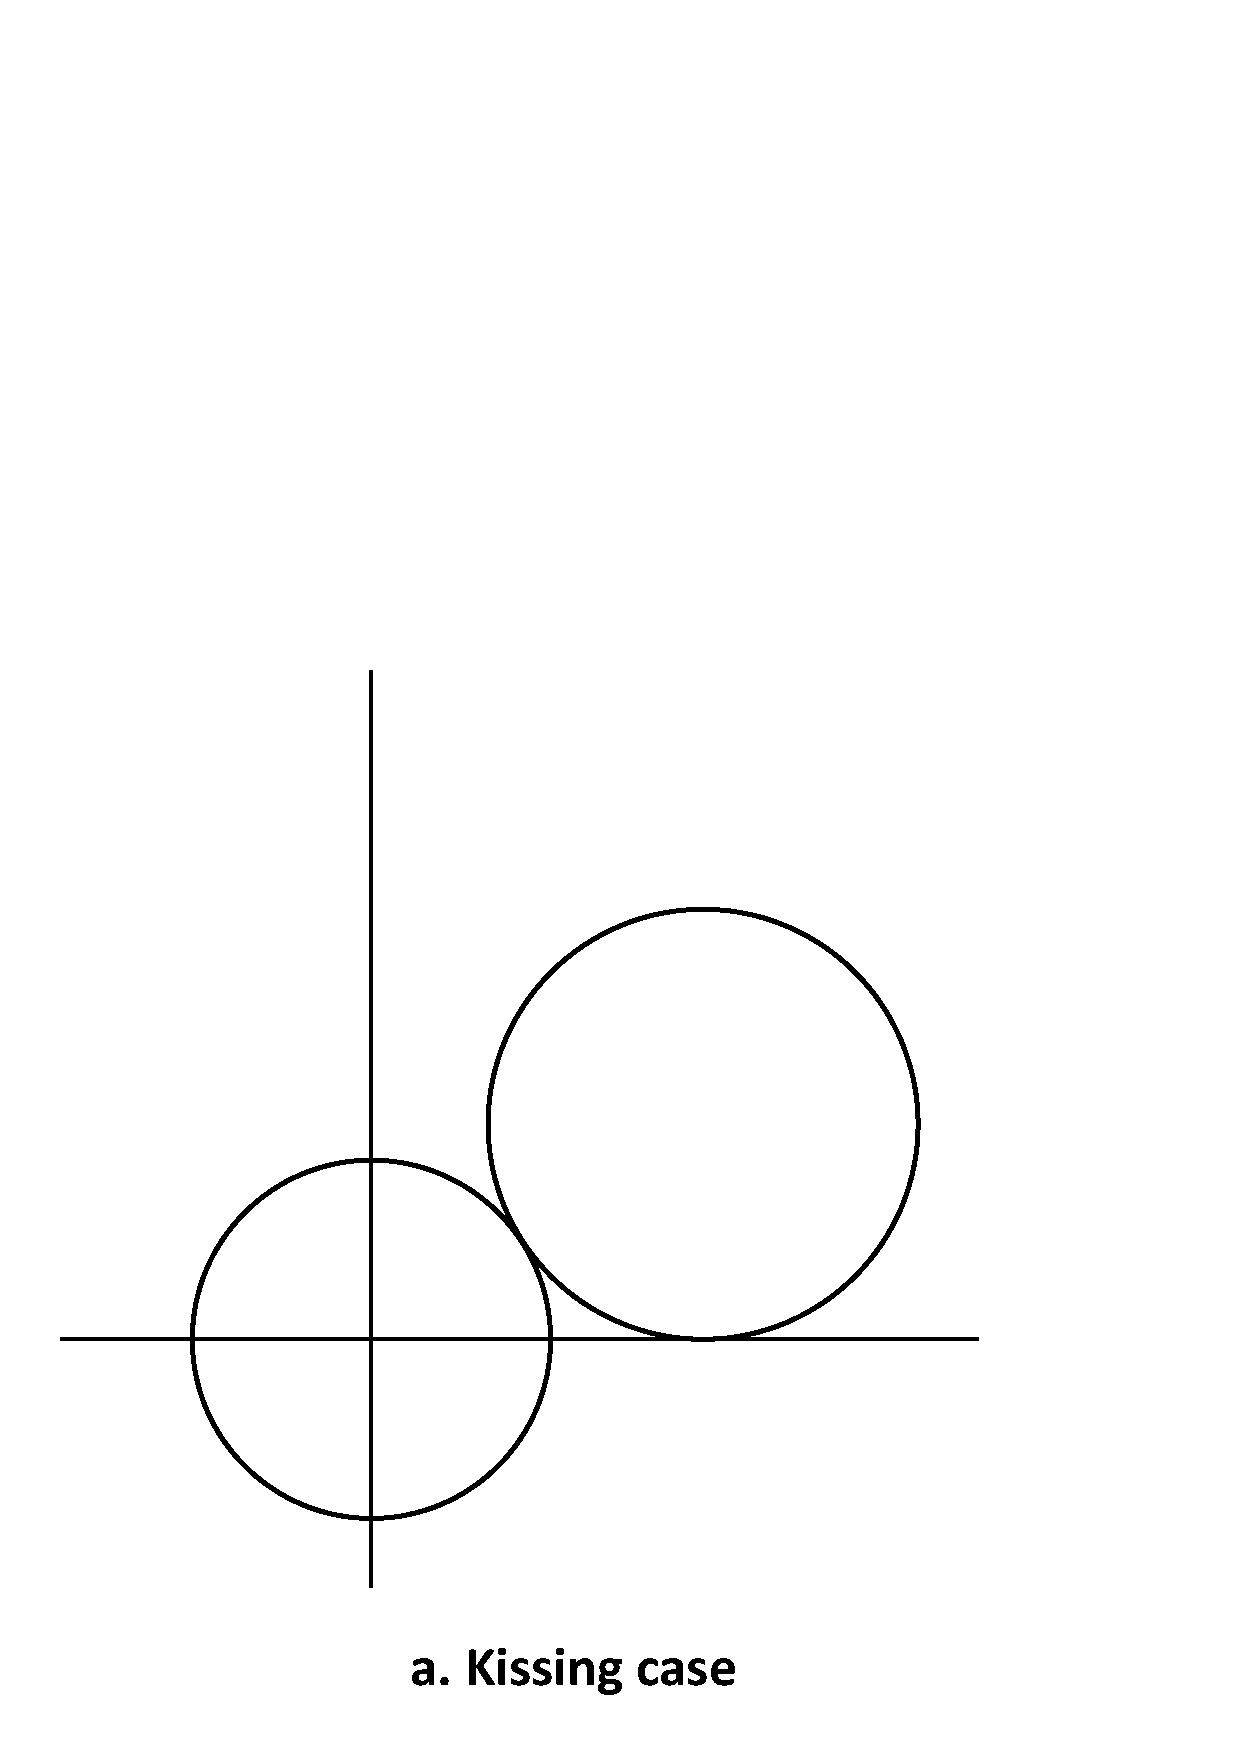
\includegraphics[height=1in,width=1.05in]{kissing.png} &
\includegraphics[height=1in,width=1.05in]{convergence.png} \\
\mbox{(a) SAT detection} &\mbox{(b) UNSAT detection} &\mbox{(c) Kissing case} & \mbox{(d) Convergent case} \\
\end{tabular}
\caption{Scenarios of solving polynomial inequations with ICP } 
\label{fig:limit} 
%\end{minipage}
\end{figure} 
\vspace{-1cm}

\suppress{%%%%
The left shows a kissing case 
$x^2 + y^2 < 2^2 \wedge (x-4)^2 + (y-3)^2 < 3^2$ such that 
$\overline{\mathbb{S}(- x^2 - y^2 + 2^2 > 0)} \cap
 \overline{\mathbb{S}(- (x-4)^2 - (y-3)^2 + 3^2 > 0)} = \{(1.6, 1.2)\}$. 
Thus, it cannot be separated by the covering by (enough small) boxes. 
%Thus, there are no coverings to separate them. 
%$x^2 + y^2 < 2^2$ and $(x-4)^2 + (y-3)^2 < 3^2$. 
The right shows a convergent case 
$y > x + \frac{1}{x} \wedge y < x \wedge x > 0$,
i.e., $xy > x^2 + x \wedge y < x \wedge x > 0$.
The latter does not appear if all intervals are bounded. 
%The open box is $(0,\infty) \times (0,\infty)$ and 
%There are no finite coverings to separate them. 
%$y > x + \frac{1}{x}$ and $y < x$ for $x > 0$.
}


\subsection{raSAT Loop}
ICP is extended to {\bf raSAT} loop~\cite{VanKhanh201227}, 
which is displayed in Algorithm~\ref{Al:raSATLoop}.  
%Fig.~\ref{fig:OTrefine}~(b). 
\begin{algorithm}[h]
\begin{algorithmic}[1]
\While {$\Pi$ is satisfiable} \Comment Some more boxes exist
\State $\pi = \{x_i \in I_{ik} \mid i \in \{1,\cdots, n\}, k \in \{1,\cdots, i_k\} \} \gets $
a solution of $\Pi$ 	
\State $B \gets $ the box represented by
$\bigwedge\limits_{i=1}^n\bigwedge\limits_{k=1}^{i_k}x_i \in I_{ik}$

\If {$B$ does not satisfy $\psi$ by using \emph{IA}}
\State $\Pi \gets \Pi \wedge \neg(\bigwedge\limits_{i=1}^n\bigwedge\limits_{k=1}^{i_k}x_i \in I_{ik})$
  \ElsIf {$B$ satisfies $\psi$ by using \emph{IA}}
\State \Return SAT
  \ElsIf {$B$ satisfies $\psi$ by using \emph{testing}} \Comment Different from ICP
\State \Return SAT
\Else \Comment Neither \emph{IA} nor \emph{testing} conclude the constraint $\implies$
\emph{Refinement} Step
\State choose $(x_i \in I_{ik}) \in \pi$ such that $\forall k_1 \in \{1,\cdots, i_k\} I_{ik} \subseteq I_{ik_1}$
\State $\{I_1, I_2\} \gets split(I_{ik})$ \Comment split $I_{ik}$
into two smaller intervals $I_1$ and $I_2$
\State $\Pi \gets \Pi \wedge (x_i \in I_{ik} \leftrightarrow (x_i \in I_1 \vee x_i \in I_2))
\wedge \neg(x_i \in I_1 \wedge x_i \in I_2)$

\EndIf
\EndWhile
\State \Return UNSAT
\end{algorithmic}
\caption{\textbf{raSAT} loop starting from the initial box
  $\Pi = \bigwedge\limits_{i=1}^n x_i \in I_i^0$}
\label{Al:raSATLoop}
\end{algorithm}
%

Its implementation {\bf raSAT} adapts various IAs including Affine Intervals
(AI)~\cite{Comba93affinearithmetic,Ngoc:2009:ORE:1685167.1685421,VanKhanh201227}
and Classical Interval (CI)~\cite{moore}.
An AI introduces noise symbols $\epsilon$'s, which are interpreted to values in $[-1,1]$. 
AIs vary depending on the treatments of the multiplication among noise symbols.
For the multiplication of the same noise symbols, $AF_2$~\cite{Messine_extensionsof}
describes by $\epsilon_+$ (or $\epsilon_{-}$), which is interpreted in $[0,1]$ (or $[-1,0]$),
and $CAI$~\cite{VanKhanh201227} describes
$\epsilon \epsilon = |\epsilon| + [-\frac{1}{4}, 0]$. 
Mostly, the product of different noise symbols are simply regarded as any value in $[-1,1]$
(e.g., $\epsilon_{\pm}$). 

Although precision is incomparable, 
an AI partially preserves the dependency among values, which is lost in CI. 
For instance, consider $x \in [2,4] = 3+\epsilon$.
Then, $x - x$ is evaluated to $[-2,2]$ by CI, where $0$ by an AI. 
%More details can be found in~\cite{VanKhanh201227}.

\begin{comment}
Affine interval introduces \emph{noise symbols} $\epsilon$, 
which are interpreted as values in $(-1,1)$. 
For instance, $x = 3 + \epsilon$ describes $x \in (2,4)$, and 
$x - x = (3 + \epsilon) - (3 + \epsilon)$ is evaluated to $0$. 
The drawback is that the multiplication without dependency might be less precise than CI.
Affine intervals also cannot represent infinite intervals, e.g., $(0,\infty)$, 
since it becomes $\infty + \infty~\epsilon$. 
Forms of Affine intervals vary by choices how to approximate multiplications. They are,
\begin{enumerate}[(i)]
\item $\epsilon \epsilon'$ is replaced with a fresh noise symbol 
($AF$)~\cite{Comba93affinearithmetic}, 
\item $\epsilon \epsilon'$ is reduced to the fixed error noise symbol 
$\epsilon_{\pm}$ ($AF_1$ and $AF_2$) \cite{Messine_extensionsof},
\item $\epsilon \epsilon'$ is replaced with $(-1,1) \epsilon$ 
(or $(-1,1) \epsilon'$) ($EAI$)~\cite{Ngoc:2009:ORE:1685167.1685421},
\item $\epsilon \epsilon$ is reduced to fixed noise symbols 
$\epsilon_+$ or $\epsilon_{-}$ ($AF_2$) \cite{Messine_extensionsof}, 
\item Chebyshev approximation of $x^2$ introduces a noise symbol $|\epsilon|$ 
as an absolute value of $\epsilon$ with 
$\epsilon \epsilon = |\epsilon| |\epsilon| = |\epsilon| + (-\frac{1}{4}, 0)$ and
$\epsilon |\epsilon| = \epsilon + (-\frac{1}{4}, \frac{1}{4})$ \cite{VanKhanh201227}. 
%(Fig.~\ref{fig:chevabs}). 
%\item keeping products of noise symbols up to degree $2$ ($\epsilon_i \epsilon_j$),
\end{enumerate} 
\end{comment}

\begin{example} \label{examp:sensitivity}
  Let $g = x^3 - 2xy$, $x = [0,2] = 1 + \epsilon_1$, and $y=[1,3] = 2+\epsilon_2$.
  $CI$ estimates the range of $g$ as $[-12,8]$, 
  $AF_2$ does 
  $-3 - \epsilon_1 - 2\epsilon_2 + 3\epsilon_+ + 3\epsilon_{\pm}$ ($= [-9,6]$), 
  and $CAI$ does 
  $[-4,-\frac{11}{4}] + [-\frac{1}{4}, 0]\epsilon_1 - 2\epsilon_2 +
  \textbf{3}|\epsilon_1| + [-2,2]\epsilon_{\pm}$ ($= [-8,4.5]$).
\end{example}


%%%%%%%%%%%%%%%%%%%%%%%%%%
\suppress{
\begin{figure}[ht]
\begin{minipage}[b]{1.0\linewidth}
\centering
\begin{tabular}{ll}
\includegraphics[height=1.6in,width=1.7in]{chev1.pdf} &
\includegraphics[height=1.6in,width=1.7in]{chev2.pdf}
\end{tabular}
\caption{Chebyshev approximation of $x^2$ and $x~|x|$}
\label{fig:chevabs}
\end{minipage}
\end{figure}

$CAI$ \cite{tapas12} consists of (ii) and (v), which keeps better precision than iv)
for multiplications of the same variables, e.g., Taylor expansion. 
%To improve precision in estimating upper and lower bounds of polynomials, we apply 
%\textbf{Affine Arithmetic} such as $AF_1$, $AF_2$ \cite{af}, $CAI$ ~\cite{tapas12} 
%instead of Classical Interval \cite{moore}. 
%Note that upper and lower bounds estimated by IA are over-approximation bounds of polynomials.
}
%%%%%%%%%%%%%%%%%%%%%%%%%%
\suppress{
\begin{definition}
%For $\exists x_1 \in (a_1,b_1) \cdots x_n \in (a_n,b_n). \bigwedge \limits_{i=1}^m f_i(x_1,\cdots,x_n) > 0$, 
Let $M = \bigwedge \limits_{i=1}^m x_i \in (a_i,b_i)$ and 
${\mathcal P} = \bigwedge \limits_{i=1}^m f_i(x_1,\cdots,x_n) > 0$. 
%
Let $\delta_i^l$ and $\delta_i^u$ be lower and upper bounds of $f_i(x_1,\cdots,x_n)$ 
estimated by IA for $x_i \in (a_i,b_i)$. Then, we say 
%
%\vspace*{0.5em}
\begin{itemize}
\item ${\mathcal P}$ is \emph{IA-VALID} under $M$, if IA evaluates 
$~\forall i \in [1,m].~\delta_i^l > 0$,
%\vspace*{0.33em}
\item ${\mathcal P}$ is \emph{IA-UNSAT} under $M$, 
$~\exists i \in [1,m].~\delta_i^u \leq 0$, and 
\item ${\mathcal P}$ is \emph{IA-SAT} under $M$, if 
$(\exists j \in [1,m].~\delta_j^l \leq 0)\; \wedge \; 
	(\bigwedge \limits_{i=1}^m \delta_i^u > 0)$.
\end{itemize} 
\end{definition}

IA-VALID and IA-UNSAT safely reason satisfiability (SAT) and unsatisfiability (UNSAT), 
respectively. However, IA-SAT cannot conclude SAT. 
}
%%%%%%%%%%%%%%%%%



\section{SAT directed Strategies of {\bf raSAT}} \label{sec:strategy}

Performance of ICP is affected by the number of variables, since the initial box 
$I_1 \times \cdots \times I_n$ may be decomposed into exponentially many boxes.
Thus, strategies for controlling a search among boxes and selecting a box / a variable
to decompose are crucial for practical efficiency. 
%%since the decomposition phase would lead exponentially large number of boxes
%%will be generated.
%The UNSAT detection requires an exhaustive search on all boxes, and
%thus finding a small UNSAT core is the key. 
%For the SAT detection, the key will be a strategic control not to fall into local optimal
%and a strategy to choose the most likely influential decomposition/box. 

\subsection{Incremental Search} \label{sec:incsearch}

Two incremental search strategies are prepared in {\bf raSAT}. 
%(1) {\em incremental widening}, and (2) {\em incremental deepening}. 

\medskip \noindent 
\textbf{Incremental Widening.}
Given $0 < \delta_0 < \delta_1 < \cdots < \delta_k = \infty$, 
{\em incremental widening} starts with 
$B_0 = [-\delta_0 , \delta_0] \times \cdots \times [-\delta_0 , \delta_0]$,
and if $\psi$ remains UNSAT, then enlarge the box to 
$B_1 = [-\delta_1 , \delta_1] \times \cdots \times [-\delta_1 , \delta_1]$.
This continues until either timeout or the result obtained. 
In {\bf raSAT}, $AF_2$ is used for $B_i$ if $i \neq k$, and $CI$ is used
for $\delta_k = \infty$. 

\begin{wrapfigure}{r}{0.4\textwidth}
%\begin{minipage}[b]{1.0\linewidth}
\vspace{-5mm}
\centering
\includegraphics[width=0.4\textwidth]{IncDeepen.png} \\
%\caption{Chebyshev approximation of $x^2$ and $x~|x|$}
\caption{Incremental Deepening}
\label{fig:incwid}
%\end{minipage}
\vspace{-3mm}
\end{wrapfigure}


\medskip\noindent 
\textbf{Incremental Deepening.}
To combine depth first and breadth first searches among decomposed boxes,
{\bf raSAT} applied {\em incremental deepening}. 
Let $\gamma_0 > \gamma_1 > \cdots > 0$. 
It applies a threshold $\gamma$, such that no more decomposition occurs 
when the size of a box becomes smaller than $\gamma$.
$\gamma$ is initially set to $\gamma_0$. 
If neither SAT nor UNSAT is detected, {\bf raSAT} restarts with the threshold $\gamma_1$
(Fig.~\ref{fig:incwid}). 
This continues until either timeout or the result obtained. 

\subsection{SAT Directed Heuristics Measure} \label{sec:SATheuristics}

%%%
\suppress{
With several hundred variables, we observe that an SMT solver works
when either SAT, or UNSAT with small UNSAT core.
%
For the latter, we need an efficient heuristics to find an UNSAT core, which is left as future work. 
For the former, the keys are how to choose variables to decompose, and 
how to choose a box to explore.
}%%%

To reduce an explosion of the number of decomposed boxes, {\bf raSAT} prepares a strategy
to select a variable at a box decomposition. 
(1) First, select a least likely satisfiable {\em API} with respect to {\em SAT-likelihood}.
(2) Then, choose a most likely influential variable in such API with respect to the 
{\em sensitivity}.
We assume an Affine interval (AI) for an interval arithmetic (IA). 

\sloppy
In line 3 of Algorithm~\ref{Al:raSATLoop},
let an AI estimate the range $range(g_j, B)$ of each polynomial $g_j$ in a box $B$
as ${[c_1,d_1]\epsilon_1 + \cdots + [c_n,d_n]\epsilon_n}$. 
Then, $range(g_j, B)$ is evaluated by instantiating $[-1,1]$ to $\epsilon_i$. 
We define
\begin{itemize} 
\item The {\em SAT-likelihood} of an API $g_j > 0$ is $| I \cap (0,\infty) | / |I|$
  for  $I = range(g_j, B)$. 
\item The {\em sensitivity} of a variable $x_i$ in an API $g_j > 0$ is $max(|c_i|, |d_i|)$. 
\end{itemize} 

\begin{example} \label{examp:SATlikelihood}
  In Example~\ref{examp:sensitivity},
  SAT-likelihood of $g$ is $0.4= \frac{6}{9-(-6)}$ by $AF_2$ 
  and $0.36 = \frac{4.5}{4.5-(-8)}$ by $CAI$.
  The sensitivity of $x$ is $1$ by $AF_2$ and $3\frac{1}{4}$ by $CAI$,
  and that of $y$ is $2$ by both.
\end{example}

Our strategy consists of three steps:
\begin{enumerate}
\item Choice of an API with the least {\em SAT likelyhood}.
\item Choice of a variable with the largest {\em sensitivity} in the API.
\item Choice of a box with the largest {\em SAT likelyhood}, where
the {\em SAT-likelihood} of a box $B$ is the least {\em SAT-likelihood} among APIs on $B$.
\end{enumerate}
The first two steps selects a variable to apply the interval decomposition and
the testdata generation. After a box decomposition is applied, the last step
compares {\em SAT-likelihood} of all boxes (including newly decomposed boxes)
to select one to explore next. 
%
At the testdata generation, 
{\bf raSAT} observes the sign of the coefficient of the noise symbol with the largest
sensitivity. 
If positive, first take the upper bound; % of possible values as the first test case;
otherwise, the lower bound. The rest is generated randomly. 

%We perform experiments only on inequations of Zankl, and Meti-Tarski families. 
The strategy is evaluated on Zankl and Meti-Tarski families of \emph{QF\_NRA}.
As a comparison with other ICP-based solvers, we compare
{\bf raSAT} with a random choice ({\em Random}), {\bf raSAT} with the strategy above
({\bf raSAT}), {\bf iSAT3}, and {\bf dReal}.

Note that (1) {\bf iSAT3} solves over $[-1000,1000]$ due to the system restriction,
while all others solve over $[-\infty, \infty]$, and (2) SAT of {\bf dReal} is 
$\delta$-SAT (SAT under tolerance of the width $\delta$); thus {\bf dReal} sometimes
answers SAT even for UNSAT problems. 
The timeout is set to 500 seconds (on Intel Xeon E5-2680v2 2.80GHz and 4GB of RAM), 
and the time shows the total of successful cases. 
% (either SAT or UNSAT). %Our combinations of strategies are,
Matrix-1, Matrix-2$\sim$5, and Meti-Tarski have 53, 96, and 4884 inequality problems resp. 

%\begin{table}[ht]
\begin{center}
\begin{tabular}{ | l | r | r | r | r | r | r | r | r |}
\hline
    \multicolumn{1}{|l|}{Benchmark} & \multicolumn{2}{c|}{\em Random} &
    \multicolumn{2}{c|}{\bf raSAT}  & \multicolumn{2}{c|}{\bf iSAT3}  &
    \multicolumn{2}{c|}{\bf dReal} \\
\hline
Matrix-1 (SAT ) & 19 & 230.39(s) & 25 & 414.99 & 11 & 4.68 & $\text{46}^{\ast}$ & 3573.43 
\\
\hline
Matrix-1 (UNSAT) & 2 & 0.01(s) & 2 & 0.01 & 3 & 0.00 & 0~ & 0.00 
\\
\hline
Matrix-2$\sim$5 (SAT) & 1 & 13.43(s) & 11 & 1264.77 & 3 & 196.40 & $\text{19}^{\ast}$ & 2708.89
\\
\hline
Matrix-2$\sim$5 (UNSAT) & 8 & 0.37(s) & 8 & 0.38 & 12 & 8.06 & 0~ & 0.00 
\\
\hline
Meti-Tarski (SAT) & 3451 & 895.14(s) & 3473 & 419.25 & 2916 & 811.53 & $\text{3523}^{\ast}$ &
441.35 
\\
\hline
Meti-Tarski (UNSAT) & 1060 & 233.46(s) & 1052 & 821.85 & 1225 & 73.83 & 1197~ & 55.39 
\\
\hline
\end{tabular}

\hfill {($\ast$ means $\delta$-SAT)} 
\end{center}
%\caption{Effectiveness of Heuristics} 
%\label{tab:rasat-experiments}
%\end{table}


%Among them the exact numbers of SAT and UNSAT problems are still unknown. 
We observe that the strategy is effective for SAT-detection in large problems, like
Matrix-2$\sim$5 (in Zankl benchmarks), which often have more than 50 variables
(Meta-Tarski has mostly less than 10 variables, and Matrix-1 has mostly less than
30 variables). 
Comparing with the state-of-the-art tool {\bf Z3 4.4} on Matrix-2$\sim$5,
the differences appear that 
{\bf Z3 4.4} solely solves Matrix-3-7, 4-12, and 5-6 (which have 75, 200, and 258 variables),
and 
{\bf raSAT} solely solves Matrix-2-3, 2-8, 3-5, 4-3, and 4-9 (which have 57, 17, 81, 139,
and 193 variables). 


\section{Extension for Equations Handling} \label{sec:eq}
\begin{comment}
For a polynomial constraint with equations,
\[\psi =
\bigwedge \limits_{j=1}^m g_j > 0 \wedge
\bigwedge \limits_{j=m+1}^{m'} g_j = 0\]
one typical way to solve equations is an algebraic method, e.g., Groebner basis.
\end{comment}
%In this section, we try a simple method based on the {\em Intermediate Value Theorem}
%which is illustrated by cases of single equation and multiple ones.

\medskip \noindent 
\textbf{Single Equation.}
A single equation (${g=0}$) can be solved by finding 2 test cases with $g > 0$ and $g < 0$.
Then, $g=0$ holds somewhere in between by the Intermediate Value Theorem.

\begin{lemma} \label{lemma:ivt}
For $\psi =
\bigwedge \limits_{j=1}^m g_j > 0~\wedge~g = 0$.
Suppose a box
$B$
and
%where
%for all $i \in \{1, \cdots, n\}$,
let ${[l_g, h_g] = range(g, B)}$, 
\begin{enumerate}[(i)]
\item If either $l_g > 0$ or $h_g < 0$, then $g = 0$ (thus $\psi$) is UNSAT in $B$. 
\item If $\bigwedge \limits_{j=1}^m g_j > 0$ is IA-valid in $B$ and there are $\vec{t},\vec{t'} \in B$
  with $g(\vec{t}) > 0$ and $g(\vec{t'}) < 0$, then $\psi$ is SAT.
\end{enumerate}
\end{lemma}

%%%%%%%%%%%%%
\suppress{
\begin{proof}
\begin{enumerate}[(i)]
\item If $l_g > 0$ or $h_g < 0$, then $g=0$ cannot be satisfied in box $I$.
  As a result, $F$ is UNSAT in $I$. 
\item If there are two instances $\vec{t},\vec{t'}$ in the box with
  $g(\vec{t}) > 0$ and $g(\vec{t'}) < 0$, it is clear from the Intermediate
  Value Theorem that there exist one point $\vec{t_0}$ between $\vec{t}$ and
  $\vec{t'}$ such that $g(\vec{t_0}) = 0$. In addition, because
  $\bigwedge \limits_{j}^m f_j > 0$ is IA-VALID in $I$, $\vec{t_0}$ also
  satisfies $\bigwedge \limits_{j}^m f_j > 0$.
  As a result, $F$ is satisfiable with $\vec{t_0}$ as the SAT instance.
\end{enumerate}
\end{proof}
}
%%%%%%%%%%%%
If neither (i) nor (ii) holds, \textbf{raSAT} continues the decomposition.
\begin{example}
  Let $\psi = f(x, y) > 0 \wedge g(x, y) = 0$.
  Suppose we find a box 
  ${B = [a, b] \times [c, d]}$
  such that $f(x, y) > 0$ is IA-valid in $B$.
  (Fig.~\ref{fig:single-equation}).
  In addition, 
  if we find two points $(u_1, v_1)$ and $(u_2, v_2)$ in $B$ such that
  $g(u_1, v_1) > 0$ and $g(u_2, v_2) < 0$,
  then the constraint is satisfiable by Lemma~\ref{lemma:ivt}. 
\end{example}


\begin{figure}
\centering
\begin{subfigure}{0.4\textwidth}
\includegraphics[width=1.\linewidth]{singleEquation.png} 
\caption{Single equation}
\label{fig:single-equation}
\end{subfigure}
\begin{subfigure}{0.4\textwidth}
\includegraphics[width=1.\linewidth]{multipleEquations.png}  
\caption{Multiple equations}
\label{fig:multiple-equations}  
\end{subfigure}
\caption{Example on solving equations using the Intermediate Value Theorem}
\end{figure}

%\medskip
\noindent 
\textbf{Multiple Equations.}
Multiple equations are solved by repeated applications of the Intermediate Value Theorem. 
Let $\bigwedge \limits_{j=1}^m g_j = 0$ and $B = {[l_1, h_1] \times \cdots [l_n, h_n]}$
with $m \leq n$. 
Let ${V = \{x_1, \cdots, x_n\}}$ be the set of variables.
For $V' = \{x_{i_1}, \cdots x_{i_k} \} \subseteq V$,
we denote $B\downarrow_{V'}$ and $B\uparrow_{V'}$ for
$\{ (r_1, \cdots, r_n) \in B \mid r_i = l_i~\text{for }i=i_1,...,i_k \}$
and ${\{ (r_1, \cdots, r_n) \in B \mid r_i = h_i~\text{for }i=i_1,...,i_k \}}$, respectively. 

\begin{definition} \label{def:CheckBasis} 
  A sequence $(V_1, \cdots, V_m)$ of subsets of $V$ is a {\em check basis} of
  $(g_1, \cdots, g_m)$ in a box $B$,
  if, for each $j,j'$ with $1 \leq j, j' \leq m$, 
\begin{enumerate}
\item $V_j (\neq \emptyset) \subseteq var(g_j)$, 
\item $V_j \cap V_{j'} = \emptyset$ if $j \neq j'$, and 
\item either $g_j > 0$ on $B\uparrow_{V_j}$ and $g_j < 0$ on $B\downarrow_{V_j}$, or
      $g_j < 0$ on $B\uparrow_{V_j}$ and $g_j > 0$ on $B\downarrow_{V_j}$. 
\end{enumerate}
\end{definition} 
%%%
\suppress{
For all $j\in \{1, \cdots, m\}$, let $k_j = |V_j|$ and
${V_j = \{v_{jk} \mid 1 \le k \le k_j \}}$, then, there exist two combinations
${(x_{j1}, \cdots, x_{jk_j}) = (t_{j1}, \cdots, t_{jk_j})}$ and
${(x_{j1}, \cdots, x_{jk_j}) = (t'_{j1}, \cdots, t'_{jk_j})}$
where $t_{jk} \neq t'_{jk} \in (l_{jk}, h_{jk})$, $1 \le k \le k_j$ such that
\[g_j(t_{j1}, \cdots, t_{jk_j}, \cdots, x_{jk}, \cdots) > 0\] and
\[g_j(t'_{j1}, \cdots, t'_{jk_j}, \cdots, x_{jk}, \cdots) < 0\]
for all values of $x_{jk}$ in $(l_{jk}, h_{jk})$ where $x_{jk} \in var(g_j) \setminus V_j$.
We denote $ivt(g_j, V_j, I)$ to represent that the polynomial $g_j$ enjoy this property
with respect to $V_j$ and $I$.
} %%%

\begin{lemma} \label{lem:multieq}
For a polynomial constraint containing multiple equations \[\psi= 
\bigwedge \limits_{j=1}^m g_j>0 \wedge
\bigwedge \limits_{j=m+1}^{m'} g_j = 0\]
and $B = {[l_1, h_1] \times \cdots [l_n, h_n]}$, 
assume that
\begin{enumerate}
\item $\bigwedge \limits_{j=1}^m g_j>0$ is IA-valid in $B$, and
\item there is a {\em check basis} $(V_{m+1}, \cdots, V_{m'})$ of $(g_{m+1}, \cdots, g_{m'})$
  in B. 
\end{enumerate}
Then, $\psi$ has a SAT instance in $B$.
\end{lemma}

The idea is, from the Intermediate Value Theorem,
each $j \in \{m+1, \cdots, m'\}$, $g_j$ has a $n - |V_{j}|$ dimensional surface of
null points of $g_j$ between $B\uparrow_{V_j}$ and $B\downarrow_{V_j}$.
Since $V_j$'s are mutually disjoint (and $g_j$' are continuous),
we have the intersection of all such surfaces of null points with
the dimension $n - \sum_{j=m+1}^{m'} |V_j|$.
Thus, this method has a limitation that 
the number of variables must be greater than or equal to the number of equations.

Fig.~\ref{fig:multiple-equations} illustrates Lemma~\ref{lem:multieq} for $m = 0$ and
$m' = n = 2$. 
The blue and red lines represent the null points of $g_1(x,y)$ and $g_2(x,y)$ in
$[c_1,d_1] \times [c_2,d_2]$, respectively.
They must have an intersection somewhere. %from the Intermediate Value Theorem. 

The table below shows preliminary experiments on benchmarks with equality constraints.
Note that Keymaera benchmark consists of 612 problems, but we do not know yet
the exact numbers of SAT and UNSAT problems 

\begin{center}
%\adjustbox{max width=\columnwidth}{}
\begin{tabular}{ | l | r | r | r | r  | r | r |}
\hline
\multicolumn{1}{|l|}{Benchmark} & \multicolumn{2}{c|}{\bf raSAT} &
\multicolumn{2}{c|}{\bf Z3 4.4} & \multicolumn{2}{c|}{\bf iSAT3}\\
\hline
Zankl (SAT) (11) & 11 & 0.07(s) & 11 & 0.17 & 0 & 0.00 \\
\hline
Zankl (UNSAT) (4) & 4 & 0.17(s) &  4 & 0.02 & 4 & 0.05 \\
\hline
Meti-Tarski (SAT) (3528)   & 875 & 174.90(s) & 1497 & 20.21 & 1 & 0.28  \\
\hline 
Meti-Tarski (UNSAT) (1573) & 781 & 401.15(s) & 1116 & 61.13 & 1075 & 22.6 \\
\hline
Keymaera (SAT)   & 0 & 0.00(s) & 0 & 0.00 & 0 & 0.00 \\
\hline
Keymaera (UNSAT) & 312 & 66.63(s) & 610 & 2.80 & 226 & 1.63\\
\hline 
\end{tabular}
\end{center}

%%%%%%
\suppress{
\begin{algorithm}
\begin{algorithmic}[1]
\Function{equationsProver}{$\bigwedge\limits_{j=k}^mg_j = 0, \Pi, V_0$}
\If {$k > m$} \Comment{All equations are checked}
	\State \Return SAT
\EndIf
\For {$V_k \in P(var(g_k))$} \Comment{$P(var(g_k))$ is the powerset of $var(g_k)$}
	\If {$V_k \cap V = \emptyset$ and $ivt(g_k, V_k, \Pi)$}
		\State $V_0 \gets V_0 \cup V_k$
		\If {\Call{equationsProver}{$\bigwedge\limits_{j=k+1}^mg_j = 0, \Pi, V_0$} = SAT}
			\State \Return SAT
		\EndIf
	\EndIf
\EndFor
\State \Return UNSAT
\EndFunction
\State \Call{equationsProver}{$\bigwedge\limits_{j=1}^mg_j = 0, \Pi, \emptyset$}
\end{algorithmic}
\caption{Solving multiple equations $\bigwedge\limits_{j=1}^m g_j = 0$ with ${\Pi = \bigwedge\limits_{i = 1}^n x_i \in (l_i, h_i)}$}
\label{Al:multiple-equations}
\end{algorithm}
}%%%%%% 




\section{Conclusion} \label{sec:conclusion and Future Work}

This paper presented an SMT solver {\bf raSAT}
for polynomial constraints
(available at {\tt http://www.jaist.ac.jp/\~{}s1310007/raSAT/index.html}), 
which aims to handle them over both reals and integers with
simple unified methodologies.
There are lots of future works and improvements, e.g., 
\begin{itemize}
\item Support mixed integers (QF\_NIRA). 
\item Implement UNSAT-directed strategies, e.g. UNSAT core.
%\item Find a good strategy for a selection of a box when solving equaltions. 
\item Set search bounds based on the cyindrical algebraic decomposition. 
\item Apply Groebner basis to overcome current limitation that the number of variables must be greater than or equal to the number of equations. 
\end{itemize}
%
\suppress{
\subsection{Observation and Discussion} 

From experimental results in Section~\ref{sec:experiments} and~\ref{sec:expsmtlib}, 
we observe the followings. 
\begin{itemize}
\item The degree of polynomials will not affect much. 
\item The number of variables are matters, but also for Z3 4.3. 
The experimental results do not show exponential growth, and we expect 
the strategy of selection of an API in which related intervals are decomposed
seems effective in practice. By observing Zankl examples, we think the maximum 
number of variables of each API seems a dominant factor. 
\item Effects of the number of APIs are not clear at the moment. In simple benchmarks, 
{\bf raSAT} is faster than Z3 4.3, however we admit that we have set small degree $n=6$
for each API. 
\end{itemize}

For instance, {\em matrix-2-all-5,8,11,12} in Zankl 
contain a long monomial (e.g., $60$) with the max degree $6$, and 
relatively many variables (e.g., $14$), which cannot be solved by Z3 4.3, but 
{\bf raSAT} does. 
As a general feeling, if an API contains more than $30 \sim 40$ variables, 
{\bf raSAT} seems saturating. 
We expect that, adding to a strategy to select an API (Section~\ref{sec:intervaldecomp}), 
we need a strategy to select variables in the focus. We expect this can be designed 
with sensitivity (Example~\ref{examp:sensitivity}) and would work in practice. 
Note that sensitivity can be used only with noise symbols in Affine intervals. 
Thus, iSAT and RSOLVER cannot use this strategy, though they are based on IA, too. 
}
%


%\balance
\bibliographystyle{splncs03}
\bibliography{generic}

\begin{thebibliography}{10}
\providecommand{\url}[1]{\texttt{#1}}
\providecommand{\urlprefix}{URL }

\bibitem{benhamou:hal-00480814}
  Benhamou, F., Granvilliers, L.: {Continuous and Interval Constraints}.
%  In: F.~Rossi, P.v.B., Walsh, T. (eds.)
  {Handbook of Constraint Programming}, 571--604. {Elsevier} (2006)

\bibitem{Barcelogic08}
Bofill, M., Nieuwenhuis, R., Oliveras, A., Rodríguez-Carbonell, E., Rubio, A.:
The Barcelogic SMT solver.
CAV 2008, LNCS5123, 294--298. (2008)

\bibitem{Bryant07decidingbit-vector}
Bryant, R.E., Kroening, D., Ouaknine, J., Seshia, S.A., Strichman, O., Brady,
B.: Deciding bit-vector arithmetic with abstraction.
TACAS 2007. 
%Lecture Notes in Computer Science, vol.
LNCS 4424,  358--372. (2007)

\bibitem{Comba93affinearithmetic}
Comba, J.L.D., Stolfi, J.: Affine arithmetic and its applications to computer
graphics. (1993)

\bibitem{smtrat}
  Corzilius, F., Loup, U., Junges, S., Ábrahám, E.: Smt-rat:
  An SMT-compliant nonlinear real arithmetic toolbox.
%In: Theory and Applications of Satisfiability Testing –
SAT 2012. LNCS 7317,  442--448. (2012)

\bibitem{isat}
Fränzle, M., Herde, C., Teige, T., Ratschan, S., Schubert, T.: Efficient
  solving of large non-linear arithmetic constraint systems with complex
  boolean structure. Journal on Satisfiability, Boolean Modeling and
  Computation  1,  209--236. (2007)

\bibitem{cordic}
Ganai, M., Ivancic, F.: Efficient decision procedure for non-linear arithmetic
constraints using cordic.
%In: Formal Methods in Computer-Aided Design, 2009.
FMCAD 2009.  61--68 {IEEE}. (2009)

\bibitem{dRealCADE13}
  Gao, S., Kong, S., Clarke, E.:
  dReal: An SMT solver for nonlinear theories over the reals.
CADE-24. LNCS 7898,  208--214. (2013)

\bibitem{Hickey:2001:IAP:502102.502106}
  Hickey, T., Ju, Q., Van~Emden, M.H.:
  Interval arithmetic: From principles to implementation.
  J. ACM  48(5),  1038--1068. (2001)

\bibitem{Jovanovic13}
  Jovanović, D., de~Moura, L.: Solving non-linear arithmetic.
  IJCAR 2012, LNCS 7364,  339--354. (2012)

\bibitem{VanKhanh201227}
Khanh, T.V., Ogawa, M.: \{SMT\} for polynomial constraints on real numbers.
TAPAS 2012, ENTCS 289, 27--40. (2012)

\bibitem{Messine_extensionsof}
Messine, F.: Extensions of affine arithmetic: Application to unconstrained
  global optimization.  J. UCS 8(11), 992-1015 (2002)

\bibitem{moore}
Moore, R.: Interval analysis. Prentice-Hall series in automatic computation,
  Prentice-Hall (1966)

\bibitem{Ngoc:2009:ORE:1685167.1685421}
Ngoc, D.T.B., Ogawa, M.: Overflow and roundoff error analysis via model
  checking. 
  SEFM 2009, 105--114, IEEE. (2009)

\bibitem{Passmore09combineddecision}
Passmore, G.O., Jackson, P.B.: Combined decision techniques for the existential
  theory of the reals. CALCULEMUS. LNCS 5625, 122--137. (2009)

\bibitem{rsolver}
Ratschan, S.: Efficient solving of quantified inequality constraints over the
  real numbers. ACM Trans. Comput. Logic  7(4),  723--748. ( 2006)

\bibitem{Zankl:2010:SNR:1939141.1939168}
Zankl, H., Middeldorp, A.: Satisfiability of non-linear (ir)rational
arithmetic. LPAR-16, LNAI 6355, 481--500. (2010)
\end{thebibliography}


\end{document}
